\documentclass{book}
\usepackage[a4paper,top=2.5cm,bottom=2.5cm,left=2.5cm,right=2.5cm]{geometry}
\usepackage{makeidx}
\usepackage{natbib}
\usepackage{graphicx}
\usepackage{multicol}
\usepackage{float}
\usepackage{listings}
\usepackage{color}
\usepackage{ifthen}
\usepackage[table]{xcolor}
\usepackage{textcomp}
\usepackage{alltt}
\usepackage{ifpdf}
\ifpdf
\usepackage[pdftex,
            pagebackref=true,
            colorlinks=true,
            linkcolor=blue,
            unicode
           ]{hyperref}
\else
\usepackage[ps2pdf,
            pagebackref=true,
            colorlinks=true,
            linkcolor=blue,
            unicode
           ]{hyperref}
\usepackage{pspicture}
\fi
\usepackage[utf8]{inputenc}
\usepackage{polski}
\usepackage[T1]{fontenc}

\usepackage{mathptmx}
\usepackage[scaled=.90]{helvet}
\usepackage{courier}
\usepackage{sectsty}
\usepackage{amssymb}
\usepackage[titles]{tocloft}
\usepackage{doxygen}
\lstset{language=C++,inputencoding=utf8,basicstyle=\footnotesize,breaklines=true,breakatwhitespace=true,tabsize=8,numbers=left }
\makeindex
\setcounter{tocdepth}{3}
\renewcommand{\footrulewidth}{0.4pt}
\renewcommand{\familydefault}{\sfdefault}
\hfuzz=15pt
\setlength{\emergencystretch}{15pt}
\hbadness=750
\tolerance=750
\begin{document}
\hypersetup{pageanchor=false,citecolor=blue}
\begin{titlepage}
\vspace*{7cm}
\begin{center}
{\Large P\-A\-M\-S\-Ilab3\-P\-O\-P\-R\-A\-W\-A }\\
\vspace*{1cm}
{\large Wygenerowano przez Doxygen 1.8.1.2}\\
\vspace*{0.5cm}
{\small So, 19 kwi 2014 15:28:14}\\
\end{center}
\end{titlepage}
\clearemptydoublepage
\pagenumbering{roman}
\tableofcontents
\clearemptydoublepage
\pagenumbering{arabic}
\hypersetup{pageanchor=true,citecolor=blue}
\chapter{Dokumentacja zadania P\-A\-M\-S\-I lab 3}
\label{index}\hypertarget{index}{}\begin{DoxyAuthor}{Autor}
Witold Zimnicki 
\end{DoxyAuthor}
\begin{DoxyDate}{Data}
19.\-4.\-2014 
\end{DoxyDate}

\chapter{Indeks klas}
\section{Hierarchia klas}
Ta lista dziedziczenia posortowana jest z grubsza, choć nie całkowicie, alfabetycznie\-:\begin{DoxyCompactList}
\item \contentsline{section}{Element\-Stosu}{\pageref{class_element_stosu}}{}
\begin{DoxyCompactList}
\item \contentsline{section}{Stos\-L}{\pageref{class_stos_l}}{}
\end{DoxyCompactList}
\item \contentsline{section}{Kolejka}{\pageref{class_kolejka}}{}
\item \contentsline{section}{Operacja}{\pageref{class_operacja}}{}
\item \contentsline{section}{Stos}{\pageref{class_stos}}{}
\item \contentsline{section}{tablica}{\pageref{classtablica}}{}
\end{DoxyCompactList}

\chapter{Indeks klas}
\section{Lista klas}
Tutaj znajdują się klasy, struktury, unie i interfejsy wraz z ich krótkimi opisami\-:\begin{DoxyCompactList}
\item\contentsline{section}{\hyperlink{class_drzewo}{Drzewo} \\*Klasa \hyperlink{class_drzewo}{Drzewo} przedstawia drzewo binarne. Sklada sie z wielu wezlow }{\pageref{class_drzewo}}{}
\item\contentsline{section}{\hyperlink{class_hash_en}{Hash\-En} \\*Klasa \hyperlink{class_hash_en}{Hash\-En} przedstawia element mapy tablicy haszujacej }{\pageref{class_hash_en}}{}
\item\contentsline{section}{\hyperlink{class_hash_m}{Hash\-M} \\*Klasa \hyperlink{class_hash_m}{Hash\-M} przechowuje w sobie elementy (klucze i wartosci) w tablicy mieszajacej }{\pageref{class_hash_m}}{}
\item\contentsline{section}{\hyperlink{class_operacja}{Operacja} \\*Deklaracja klasy \hyperlink{class_operacja}{Operacja} }{\pageref{class_operacja}}{}
\item\contentsline{section}{\hyperlink{class_wezel}{Wezel} \\*Klasa \hyperlink{class_wezel}{Wezel} opisuje obiekt bedacy elementem wiekszej klasy \hyperlink{class_drzewo}{Drzewo} -\/ drzewa binarnego. Posiada on swoj klucz -\/ string, oraz wartosc -\/ int }{\pageref{class_wezel}}{}
\end{DoxyCompactList}

\chapter{Indeks plików}
\section{Lista plików}
Tutaj znajduje się lista wszystkich plików z ich krótkimi opisami\-:\begin{DoxyCompactList}
\item\contentsline{section}{/home/karolina/\-Pulpit/\-Project41\-Poker(1)/\-Project41\-Poker/\-Project41\-Poker/prj/inc/\hyperlink{_c_p_u_8h}{C\-P\-U.\-h} \\*Definicja klasy \hyperlink{class_c_p_u}{C\-P\-U} }{\pageref{_c_p_u_8h}}{}
\item\contentsline{section}{/home/karolina/\-Pulpit/\-Project41\-Poker(1)/\-Project41\-Poker/\-Project41\-Poker/prj/inc/\hyperlink{_g_r_a_8h}{G\-R\-A.\-h} \\*Definicja klasy \hyperlink{class_g_r_a}{G\-R\-A} }{\pageref{_g_r_a_8h}}{}
\item\contentsline{section}{/home/karolina/\-Pulpit/\-Project41\-Poker(1)/\-Project41\-Poker/\-Project41\-Poker/prj/inc/\hyperlink{gracz_8h}{gracz.\-h} \\*Definicja klasy \hyperlink{class_gracz}{Gracz} }{\pageref{gracz_8h}}{}
\item\contentsline{section}{/home/karolina/\-Pulpit/\-Project41\-Poker(1)/\-Project41\-Poker/\-Project41\-Poker/prj/inc/\hyperlink{interfejs_8h}{interfejs.\-h} \\*Definicja klasy \hyperlink{class_interfejs}{Interfejs} }{\pageref{interfejs_8h}}{}
\item\contentsline{section}{/home/karolina/\-Pulpit/\-Project41\-Poker(1)/\-Project41\-Poker/\-Project41\-Poker/prj/inc/\hyperlink{karta_8h}{karta.\-h} \\*Definicja klasy \hyperlink{class_karta}{Karta} }{\pageref{karta_8h}}{}
\item\contentsline{section}{/home/karolina/\-Pulpit/\-Project41\-Poker(1)/\-Project41\-Poker/\-Project41\-Poker/prj/inc/\hyperlink{talia_8h}{talia.\-h} \\*Definicja klasy \hyperlink{class_talia}{Talia} }{\pageref{talia_8h}}{}
\item\contentsline{section}{/home/karolina/\-Pulpit/\-Project41\-Poker(1)/\-Project41\-Poker/\-Project41\-Poker/prj/inc/\hyperlink{zestaw_8h}{zestaw.\-h} \\*Definicja klasy \hyperlink{class_zestaw}{Zestaw} }{\pageref{zestaw_8h}}{}
\item\contentsline{section}{/home/karolina/\-Pulpit/\-Project41\-Poker(1)/\-Project41\-Poker/\-Project41\-Poker/prj/src/\hyperlink{_c_p_u_8cpp}{C\-P\-U.\-cpp} \\*Definicja metody klasy \hyperlink{class_c_p_u}{C\-P\-U} }{\pageref{_c_p_u_8cpp}}{}
\item\contentsline{section}{/home/karolina/\-Pulpit/\-Project41\-Poker(1)/\-Project41\-Poker/\-Project41\-Poker/prj/src/\hyperlink{_g_r_a_8cpp}{G\-R\-A.\-cpp} \\*Definicja metody klasy \hyperlink{class_g_r_a}{G\-R\-A} }{\pageref{_g_r_a_8cpp}}{}
\item\contentsline{section}{/home/karolina/\-Pulpit/\-Project41\-Poker(1)/\-Project41\-Poker/\-Project41\-Poker/prj/src/\hyperlink{gracz_8cpp}{gracz.\-cpp} \\*Definicja metody klasy \hyperlink{class_gracz}{Gracz} }{\pageref{gracz_8cpp}}{}
\item\contentsline{section}{/home/karolina/\-Pulpit/\-Project41\-Poker(1)/\-Project41\-Poker/\-Project41\-Poker/prj/src/\hyperlink{interfejs_8cpp}{interfejs.\-cpp} \\*Definicja metody klasy \hyperlink{class_interfejs}{Interfejs} }{\pageref{interfejs_8cpp}}{}
\item\contentsline{section}{/home/karolina/\-Pulpit/\-Project41\-Poker(1)/\-Project41\-Poker/\-Project41\-Poker/prj/src/\hyperlink{karta_8cpp}{karta.\-cpp} \\*Definicja metody klasy \hyperlink{class_karta}{Karta} }{\pageref{karta_8cpp}}{}
\item\contentsline{section}{/home/karolina/\-Pulpit/\-Project41\-Poker(1)/\-Project41\-Poker/\-Project41\-Poker/prj/src/\hyperlink{main_8cpp}{main.\-cpp} \\*Plik glowny programu }{\pageref{main_8cpp}}{}
\item\contentsline{section}{/home/karolina/\-Pulpit/\-Project41\-Poker(1)/\-Project41\-Poker/\-Project41\-Poker/prj/src/\hyperlink{talia_8cpp}{talia.\-cpp} \\*Definicja metody klasy \hyperlink{class_talia}{Talia} }{\pageref{talia_8cpp}}{}
\item\contentsline{section}{/home/karolina/\-Pulpit/\-Project41\-Poker(1)/\-Project41\-Poker/\-Project41\-Poker/prj/src/\hyperlink{zestaw_8cpp}{zestaw.\-cpp} \\*Definicja metody klasy \hyperlink{class_zestaw}{Zestaw} }{\pageref{zestaw_8cpp}}{}
\end{DoxyCompactList}

\chapter{Dokumentacja klas}
\hypertarget{class_element_stosu}{\section{Dokumentacja klasy Element\-Stosu}
\label{class_element_stosu}\index{Element\-Stosu@{Element\-Stosu}}
}


Definicja klasy \hyperlink{class_element_stosu}{Element\-Stosu} , opisujacej jeden z listowej implementacji klasy \hyperlink{class_stos_l}{Stos\-L}.  




{\ttfamily \#include $<$Stos\-L.\-h$>$}

Diagram dziedziczenia dla Element\-Stosu\begin{figure}[H]
\begin{center}
\leavevmode
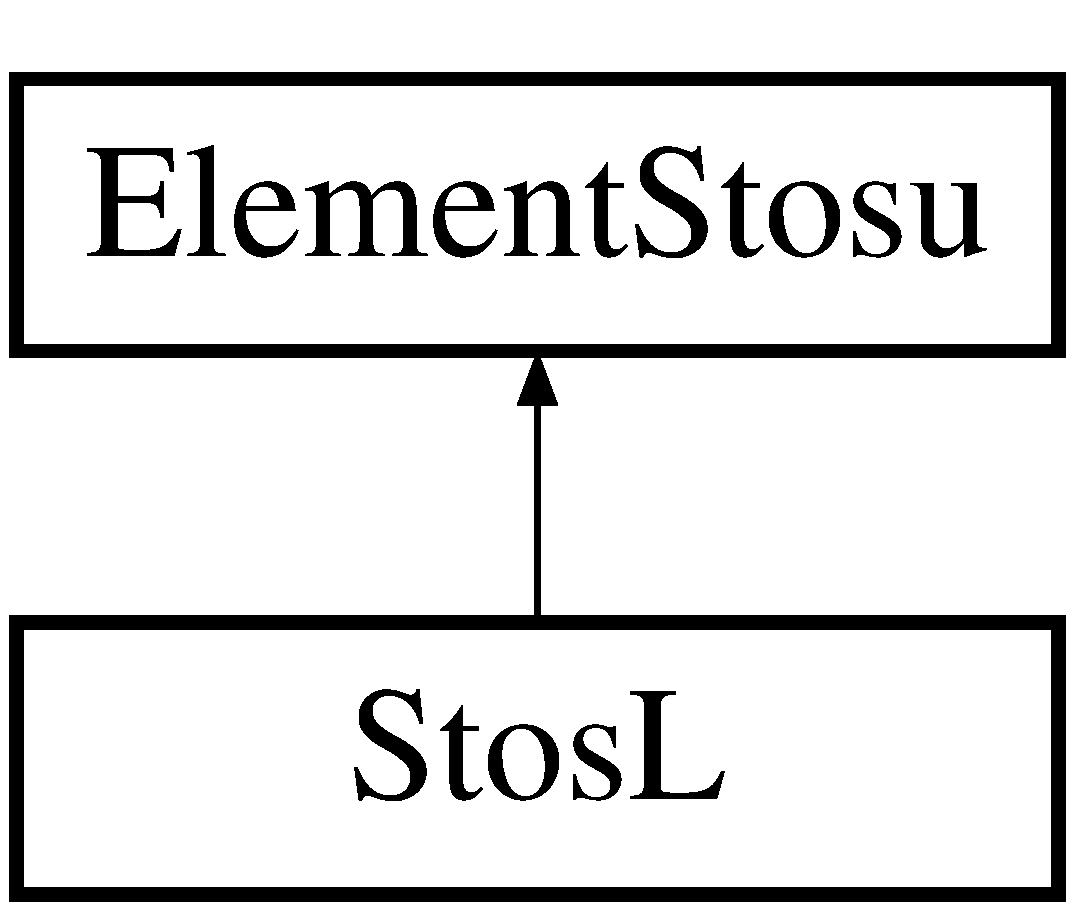
\includegraphics[height=2.000000cm]{class_element_stosu}
\end{center}
\end{figure}
\subsection*{Metody publiczne}
\begin{DoxyCompactItemize}
\item 
\hyperlink{class_element_stosu_a0ee1750bbb83a84d1a73459d4f39897d}{Element\-Stosu} ()
\begin{DoxyCompactList}\small\item\em Konstruktor klasy \hyperlink{class_element_stosu}{Element\-Stosu}. \end{DoxyCompactList}\end{DoxyCompactItemize}
\subsection*{Atrybuty publiczne}
\begin{DoxyCompactItemize}
\item 
int \hyperlink{class_element_stosu_a78ebcb4f6af82fdcab2d8b458c4f05ab}{wartosc}
\begin{DoxyCompactList}\small\item\em Pole przechowujace wartosc tego elementu. \end{DoxyCompactList}\item 
\hyperlink{class_element_stosu}{Element\-Stosu} $\ast$ \hyperlink{class_element_stosu_a2f7c031eb0456369bac68a02c030601d}{nastepny}
\begin{DoxyCompactList}\small\item\em Wskaznik na nastepny element. \end{DoxyCompactList}\end{DoxyCompactItemize}


\subsection{Opis szczegółowy}
Definicja klasy \hyperlink{class_element_stosu}{Element\-Stosu} , opisujacej jeden z listowej implementacji klasy \hyperlink{class_stos_l}{Stos\-L}. 

\subsection{Dokumentacja konstruktora i destruktora}
\hypertarget{class_element_stosu_a0ee1750bbb83a84d1a73459d4f39897d}{\index{Element\-Stosu@{Element\-Stosu}!Element\-Stosu@{Element\-Stosu}}
\index{Element\-Stosu@{Element\-Stosu}!ElementStosu@{Element\-Stosu}}
\subsubsection[{Element\-Stosu}]{\setlength{\rightskip}{0pt plus 5cm}Element\-Stosu\-::\-Element\-Stosu (
\begin{DoxyParamCaption}
{}
\end{DoxyParamCaption}
)}}\label{class_element_stosu_a0ee1750bbb83a84d1a73459d4f39897d}


Konstruktor klasy \hyperlink{class_element_stosu}{Element\-Stosu}. 

Konstruktor ustawia wskaznik nastepnego elementu na zero (poniewaz na poczatku nie ma zadnych elementow). 

\subsection{Dokumentacja atrybutów składowych}
\hypertarget{class_element_stosu_a2f7c031eb0456369bac68a02c030601d}{\index{Element\-Stosu@{Element\-Stosu}!nastepny@{nastepny}}
\index{nastepny@{nastepny}!ElementStosu@{Element\-Stosu}}
\subsubsection[{nastepny}]{\setlength{\rightskip}{0pt plus 5cm}{\bf Element\-Stosu}$\ast$ Element\-Stosu\-::nastepny}}\label{class_element_stosu_a2f7c031eb0456369bac68a02c030601d}


Wskaznik na nastepny element. 

\hypertarget{class_element_stosu_a78ebcb4f6af82fdcab2d8b458c4f05ab}{\index{Element\-Stosu@{Element\-Stosu}!wartosc@{wartosc}}
\index{wartosc@{wartosc}!ElementStosu@{Element\-Stosu}}
\subsubsection[{wartosc}]{\setlength{\rightskip}{0pt plus 5cm}int Element\-Stosu\-::wartosc}}\label{class_element_stosu_a78ebcb4f6af82fdcab2d8b458c4f05ab}


Pole przechowujace wartosc tego elementu. 



Dokumentacja dla tej klasy została wygenerowana z plików\-:\begin{DoxyCompactItemize}
\item 
C\-:/\-Users/\-Witek/\-Documents/\-Visual Studio 2012/\-Projects/\-Project44\-P\-A\-M\-S\-Ilab3/\-Project44\-P\-A\-M\-S\-Ilab3/\hyperlink{_stos_l_8h}{Stos\-L.\-h}\item 
C\-:/\-Users/\-Witek/\-Documents/\-Visual Studio 2012/\-Projects/\-Project44\-P\-A\-M\-S\-Ilab3/\-Project44\-P\-A\-M\-S\-Ilab3/\hyperlink{_stos_l_8cpp}{Stos\-L.\-cpp}\end{DoxyCompactItemize}

\hypertarget{class_kolejka}{\section{Dokumentacja klasy Kolejka}
\label{class_kolejka}\index{Kolejka@{Kolejka}}
}


Definicja klasy \hyperlink{class_kolejka}{Kolejka}.  




{\ttfamily \#include $<$Kolejka.\-h$>$}

\subsection*{Metody publiczne}
\begin{DoxyCompactItemize}
\item 
\hyperlink{class_kolejka_a37c886fdc73dce62b04da0381dec5484}{Kolejka} ()
\begin{DoxyCompactList}\small\item\em Konstruktor domyslny klasy \hyperlink{class_kolejka}{Kolejka}. \end{DoxyCompactList}\item 
\hyperlink{class_kolejka_a507889c5f122d922544fdaf4dd58b2d0}{Kolejka} (int Ilosc)
\begin{DoxyCompactList}\small\item\em Konstruktor pobierajacy parametr ilosci elementow tablicy. \end{DoxyCompactList}\item 
\hyperlink{class_kolejka_a352f86ff08cd47be6c35c60bb0f873a6}{$\sim$\-Kolejka} ()
\begin{DoxyCompactList}\small\item\em Destruktor usuwajacy tablice dynamiczna Q. \end{DoxyCompactList}\item 
bool \hyperlink{class_kolejka_afdd931c17c1fa4d93bc5c8aa45cb212a}{empty} ()
\begin{DoxyCompactList}\small\item\em Funkcja sprawdzajaca, czy tablica jest pusta. \end{DoxyCompactList}\item 
int \hyperlink{class_kolejka_a6476787f1d02eb82e334f1be10daea66}{front} ()
\begin{DoxyCompactList}\small\item\em Funkcja zwraca element na koncu kolejki. \end{DoxyCompactList}\item 
void \hyperlink{class_kolejka_a5f21d536bde87ae387e23e52ca27e3f9}{enqueue} (int element)
\begin{DoxyCompactList}\small\item\em Funkcja kolejkuje wybrany element. \end{DoxyCompactList}\item 
void \hyperlink{class_kolejka_a9c78c81b3ef4d4d7a54215ab7fe380ff}{dequeue} ()
\begin{DoxyCompactList}\small\item\em Funkcja usuwa ostatni element kolejki. \end{DoxyCompactList}\item 
void \hyperlink{class_kolejka_a555c767a2f9afd38aa60773ea9b62419}{Wyswietl} ()
\begin{DoxyCompactList}\small\item\em Funkcja wyswietla cala kolejke. \end{DoxyCompactList}\item 
void \hyperlink{class_kolejka_a8def296b0c464119e80a96258785b123}{Ustal\-Rozmiar} (int roz)
\begin{DoxyCompactList}\small\item\em Funkcja przypisuje wybrany rozmiar kolejce. \end{DoxyCompactList}\end{DoxyCompactItemize}


\subsection{Opis szczegółowy}
Definicja klasy \hyperlink{class_kolejka}{Kolejka}. 

Ta struktura danych pozwala na zapisywanie danych do kolejki zaimplementowej tablicowo. 

\subsection{Dokumentacja konstruktora i destruktora}
\hypertarget{class_kolejka_a37c886fdc73dce62b04da0381dec5484}{\index{Kolejka@{Kolejka}!Kolejka@{Kolejka}}
\index{Kolejka@{Kolejka}!Kolejka@{Kolejka}}
\subsubsection[{Kolejka}]{\setlength{\rightskip}{0pt plus 5cm}Kolejka\-::\-Kolejka (
\begin{DoxyParamCaption}
{}
\end{DoxyParamCaption}
)}}\label{class_kolejka_a37c886fdc73dce62b04da0381dec5484}


Konstruktor domyslny klasy \hyperlink{class_kolejka}{Kolejka}. 

\hypertarget{class_kolejka_a507889c5f122d922544fdaf4dd58b2d0}{\index{Kolejka@{Kolejka}!Kolejka@{Kolejka}}
\index{Kolejka@{Kolejka}!Kolejka@{Kolejka}}
\subsubsection[{Kolejka}]{\setlength{\rightskip}{0pt plus 5cm}Kolejka\-::\-Kolejka (
\begin{DoxyParamCaption}
\item[{int}]{Ilosc}
\end{DoxyParamCaption}
)}}\label{class_kolejka_a507889c5f122d922544fdaf4dd58b2d0}


Konstruktor pobierajacy parametr ilosci elementow tablicy. 

wskpocz po utworzeniu zmiennej klasy \hyperlink{class_kolejka}{Kolejka} pokazuje na poczatek tablicy.

Parametry i najwazniejsza pola funkcji\-: -\/\-Ilosc\-: parametr okresla rozmiar stworzonej tablicy kolejki. \hypertarget{class_kolejka_a352f86ff08cd47be6c35c60bb0f873a6}{\index{Kolejka@{Kolejka}!$\sim$\-Kolejka@{$\sim$\-Kolejka}}
\index{$\sim$\-Kolejka@{$\sim$\-Kolejka}!Kolejka@{Kolejka}}
\subsubsection[{$\sim$\-Kolejka}]{\setlength{\rightskip}{0pt plus 5cm}Kolejka\-::$\sim$\-Kolejka (
\begin{DoxyParamCaption}
{}
\end{DoxyParamCaption}
)}}\label{class_kolejka_a352f86ff08cd47be6c35c60bb0f873a6}


Destruktor usuwajacy tablice dynamiczna Q. 



\subsection{Dokumentacja funkcji składowych}
\hypertarget{class_kolejka_a9c78c81b3ef4d4d7a54215ab7fe380ff}{\index{Kolejka@{Kolejka}!dequeue@{dequeue}}
\index{dequeue@{dequeue}!Kolejka@{Kolejka}}
\subsubsection[{dequeue}]{\setlength{\rightskip}{0pt plus 5cm}void Kolejka\-::dequeue (
\begin{DoxyParamCaption}
{}
\end{DoxyParamCaption}
)}}\label{class_kolejka_a9c78c81b3ef4d4d7a54215ab7fe380ff}


Funkcja usuwa ostatni element kolejki. 

\hypertarget{class_kolejka_afdd931c17c1fa4d93bc5c8aa45cb212a}{\index{Kolejka@{Kolejka}!empty@{empty}}
\index{empty@{empty}!Kolejka@{Kolejka}}
\subsubsection[{empty}]{\setlength{\rightskip}{0pt plus 5cm}bool Kolejka\-::empty (
\begin{DoxyParamCaption}
{}
\end{DoxyParamCaption}
)}}\label{class_kolejka_afdd931c17c1fa4d93bc5c8aa45cb212a}


Funkcja sprawdzajaca, czy tablica jest pusta. 

\begin{DoxyReturn}{Zwraca}
prawde, jesli kolejka jest pusta; falsz, jesli kolejka posiada elementy 
\end{DoxyReturn}
\hypertarget{class_kolejka_a5f21d536bde87ae387e23e52ca27e3f9}{\index{Kolejka@{Kolejka}!enqueue@{enqueue}}
\index{enqueue@{enqueue}!Kolejka@{Kolejka}}
\subsubsection[{enqueue}]{\setlength{\rightskip}{0pt plus 5cm}void Kolejka\-::enqueue (
\begin{DoxyParamCaption}
\item[{int}]{element}
\end{DoxyParamCaption}
)}}\label{class_kolejka_a5f21d536bde87ae387e23e52ca27e3f9}


Funkcja kolejkuje wybrany element. 

Parametry i najwazniejsza pola funkcji\-: -\/element\-: liczba typu int, ktora chcemy zakolejkowac.

Gdy liczba elementow jest wieksza badz rowna rozmiarowi kolejki, nic sie nie dzieje. \hypertarget{class_kolejka_a6476787f1d02eb82e334f1be10daea66}{\index{Kolejka@{Kolejka}!front@{front}}
\index{front@{front}!Kolejka@{Kolejka}}
\subsubsection[{front}]{\setlength{\rightskip}{0pt plus 5cm}int Kolejka\-::front (
\begin{DoxyParamCaption}
{}
\end{DoxyParamCaption}
)}}\label{class_kolejka_a6476787f1d02eb82e334f1be10daea66}


Funkcja zwraca element na koncu kolejki. 

\begin{DoxyReturn}{Zwraca}
ostatni element kolejki, gdy posiada elementy; falsz, gdy ich nie posiada. 
\end{DoxyReturn}
\hypertarget{class_kolejka_a8def296b0c464119e80a96258785b123}{\index{Kolejka@{Kolejka}!Ustal\-Rozmiar@{Ustal\-Rozmiar}}
\index{Ustal\-Rozmiar@{Ustal\-Rozmiar}!Kolejka@{Kolejka}}
\subsubsection[{Ustal\-Rozmiar}]{\setlength{\rightskip}{0pt plus 5cm}void Kolejka\-::\-Ustal\-Rozmiar (
\begin{DoxyParamCaption}
\item[{int}]{roz}
\end{DoxyParamCaption}
)}}\label{class_kolejka_a8def296b0c464119e80a96258785b123}


Funkcja przypisuje wybrany rozmiar kolejce. 

\hypertarget{class_kolejka_a555c767a2f9afd38aa60773ea9b62419}{\index{Kolejka@{Kolejka}!Wyswietl@{Wyswietl}}
\index{Wyswietl@{Wyswietl}!Kolejka@{Kolejka}}
\subsubsection[{Wyswietl}]{\setlength{\rightskip}{0pt plus 5cm}void Kolejka\-::\-Wyswietl (
\begin{DoxyParamCaption}
{}
\end{DoxyParamCaption}
)}}\label{class_kolejka_a555c767a2f9afd38aa60773ea9b62419}


Funkcja wyswietla cala kolejke. 



Dokumentacja dla tej klasy została wygenerowana z plików\-:\begin{DoxyCompactItemize}
\item 
C\-:/\-Users/\-Witek/\-Documents/\-Visual Studio 2012/\-Projects/\-Project45\-P\-A\-M\-S\-Ilab5/\-Project45\-P\-A\-M\-S\-Ilab5/\hyperlink{_kolejka_8h}{Kolejka.\-h}\item 
C\-:/\-Users/\-Witek/\-Documents/\-Visual Studio 2012/\-Projects/\-Project45\-P\-A\-M\-S\-Ilab5/\-Project45\-P\-A\-M\-S\-Ilab5/\hyperlink{_kolejka_8cpp}{Kolejka.\-cpp}\end{DoxyCompactItemize}

\hypertarget{class_operacja}{\section{Dokumentacja klasy Operacja}
\label{class_operacja}\index{Operacja@{Operacja}}
}


Deklaracja klasy \hyperlink{class_operacja}{Operacja}.  




{\ttfamily \#include $<$operacja.\-h$>$}

\subsection*{Metody publiczne}
\begin{DoxyCompactItemize}
\item 
void \hyperlink{class_operacja_a8a31476894d307c400f965dd3dfcbb46}{Zmierz\-Czas\-Start} ()
\begin{DoxyCompactList}\small\item\em Funkcja wyznaczajaca poczatek pomiaru czasu. \end{DoxyCompactList}\item 
void \hyperlink{class_operacja_a971e3493bec71fc140ac44f74bd92998}{Zmierz\-Czas\-Koniec\-Drzewo} ()
\begin{DoxyCompactList}\small\item\em Funkcja wyznaczajaca koniec pomiaru czasu dla zapelniania drzewa binarnego. \end{DoxyCompactList}\item 
void \hyperlink{class_operacja_a39ea8e62797c94693c75abe6f0416035}{Zmierz\-Czas\-Koniec\-Hasz} ()
\begin{DoxyCompactList}\small\item\em Funkcja wyznaczajaca koniec pomiaru czasu dla zapelniania tablicy haszujacej. \end{DoxyCompactList}\item 
void \hyperlink{class_operacja_a3f6cb38d924c260711fad70fe0eed35f}{Pobierz\-Ilosc\-Powtorzen} ()
\begin{DoxyCompactList}\small\item\em Funkcja pobierajaca ilosc powtorzen od uzytkownika. \end{DoxyCompactList}\item 
void \hyperlink{class_operacja_aca61c478012e3477b123b1cccedd375c}{Policz\-Operacje\-Drzewo} ()
\begin{DoxyCompactList}\small\item\em Funkcja wykonujaca zapelnianie drzewa binarnego. \end{DoxyCompactList}\item 
void \hyperlink{class_operacja_a97f0315ebc8d718a497415023ef11564}{Policz\-Operacje\-Hasz} ()
\begin{DoxyCompactList}\small\item\em Funkcja wykonujaca zapelnianie tablicy haszujacej. \end{DoxyCompactList}\item 
void \hyperlink{class_operacja_add48398ebfeae90a0d1b58a31962fd7d}{Dzialaj} ()
\begin{DoxyCompactList}\small\item\em Glowna Funkcja Operacji wykonujaca wszystkie potrzebne funkcje do uzyskania czasow. \end{DoxyCompactList}\item 
\hyperlink{class_operacja_a1624fb5817c0b60e1680509fc4517732}{Operacja} ()
\begin{DoxyCompactList}\small\item\em Konstruktor bezparametryczny. \end{DoxyCompactList}\end{DoxyCompactItemize}
\subsection*{Atrybuty publiczne}
\begin{DoxyCompactItemize}
\item 
\hyperlink{class_hash_m}{Hash\-M} \hyperlink{class_operacja_ad67a2aa20b71ec0e1f1cff12b7220b6a}{haszujaca}
\begin{DoxyCompactList}\small\item\em Tablica haszujaca dla danej operacji. \end{DoxyCompactList}\item 
\hyperlink{class_drzewo}{Drzewo} \hyperlink{class_operacja_a814e223e988958ccbbe66aef89054da3}{drzewko}
\begin{DoxyCompactList}\small\item\em \hyperlink{class_drzewo}{Drzewo} binarne dla danej operacji. \end{DoxyCompactList}\item 
int \hyperlink{class_operacja_aa568b17d05f31132b3d97eb5b7e93d61}{Powtorzenia}
\begin{DoxyCompactList}\small\item\em Pole przechowujace informiacji o ilosci powtorzen dla danej operacji. \end{DoxyCompactList}\end{DoxyCompactItemize}


\subsection{Opis szczegółowy}
Deklaracja klasy \hyperlink{class_operacja}{Operacja}. 

Klasa \hyperlink{class_operacja}{Operacja} posiada pola oraz funkcje potrzebne do wykonywania dzialan na roznych strukturach danych. 

\subsection{Dokumentacja konstruktora i destruktora}
\hypertarget{class_operacja_a1624fb5817c0b60e1680509fc4517732}{\index{Operacja@{Operacja}!Operacja@{Operacja}}
\index{Operacja@{Operacja}!Operacja@{Operacja}}
\subsubsection[{Operacja}]{\setlength{\rightskip}{0pt plus 5cm}Operacja\-::\-Operacja (
\begin{DoxyParamCaption}
{}
\end{DoxyParamCaption}
)}}\label{class_operacja_a1624fb5817c0b60e1680509fc4517732}


Konstruktor bezparametryczny. 

Konstruktor pobiera wybrana ilosc zestawow, ktore chcemy dodac do tablicy i drzewa. 

\subsection{Dokumentacja funkcji składowych}
\hypertarget{class_operacja_add48398ebfeae90a0d1b58a31962fd7d}{\index{Operacja@{Operacja}!Dzialaj@{Dzialaj}}
\index{Dzialaj@{Dzialaj}!Operacja@{Operacja}}
\subsubsection[{Dzialaj}]{\setlength{\rightskip}{0pt plus 5cm}void Operacja\-::\-Dzialaj (
\begin{DoxyParamCaption}
{}
\end{DoxyParamCaption}
)}}\label{class_operacja_add48398ebfeae90a0d1b58a31962fd7d}


Glowna Funkcja Operacji wykonujaca wszystkie potrzebne funkcje do uzyskania czasow. 

\hypertarget{class_operacja_a3f6cb38d924c260711fad70fe0eed35f}{\index{Operacja@{Operacja}!Pobierz\-Ilosc\-Powtorzen@{Pobierz\-Ilosc\-Powtorzen}}
\index{Pobierz\-Ilosc\-Powtorzen@{Pobierz\-Ilosc\-Powtorzen}!Operacja@{Operacja}}
\subsubsection[{Pobierz\-Ilosc\-Powtorzen}]{\setlength{\rightskip}{0pt plus 5cm}void Operacja\-::\-Pobierz\-Ilosc\-Powtorzen (
\begin{DoxyParamCaption}
{}
\end{DoxyParamCaption}
)}}\label{class_operacja_a3f6cb38d924c260711fad70fe0eed35f}


Funkcja pobierajaca ilosc powtorzen od uzytkownika. 

\hypertarget{class_operacja_aca61c478012e3477b123b1cccedd375c}{\index{Operacja@{Operacja}!Policz\-Operacje\-Drzewo@{Policz\-Operacje\-Drzewo}}
\index{Policz\-Operacje\-Drzewo@{Policz\-Operacje\-Drzewo}!Operacja@{Operacja}}
\subsubsection[{Policz\-Operacje\-Drzewo}]{\setlength{\rightskip}{0pt plus 5cm}void Operacja\-::\-Policz\-Operacje\-Drzewo (
\begin{DoxyParamCaption}
{}
\end{DoxyParamCaption}
)}}\label{class_operacja_aca61c478012e3477b123b1cccedd375c}


Funkcja wykonujaca zapelnianie drzewa binarnego. 

\hypertarget{class_operacja_a97f0315ebc8d718a497415023ef11564}{\index{Operacja@{Operacja}!Policz\-Operacje\-Hasz@{Policz\-Operacje\-Hasz}}
\index{Policz\-Operacje\-Hasz@{Policz\-Operacje\-Hasz}!Operacja@{Operacja}}
\subsubsection[{Policz\-Operacje\-Hasz}]{\setlength{\rightskip}{0pt plus 5cm}void Operacja\-::\-Policz\-Operacje\-Hasz (
\begin{DoxyParamCaption}
{}
\end{DoxyParamCaption}
)}}\label{class_operacja_a97f0315ebc8d718a497415023ef11564}


Funkcja wykonujaca zapelnianie tablicy haszujacej. 

\hypertarget{class_operacja_a971e3493bec71fc140ac44f74bd92998}{\index{Operacja@{Operacja}!Zmierz\-Czas\-Koniec\-Drzewo@{Zmierz\-Czas\-Koniec\-Drzewo}}
\index{Zmierz\-Czas\-Koniec\-Drzewo@{Zmierz\-Czas\-Koniec\-Drzewo}!Operacja@{Operacja}}
\subsubsection[{Zmierz\-Czas\-Koniec\-Drzewo}]{\setlength{\rightskip}{0pt plus 5cm}void Operacja\-::\-Zmierz\-Czas\-Koniec\-Drzewo (
\begin{DoxyParamCaption}
{}
\end{DoxyParamCaption}
)}}\label{class_operacja_a971e3493bec71fc140ac44f74bd92998}


Funkcja wyznaczajaca koniec pomiaru czasu dla zapelniania drzewa binarnego. 

\hypertarget{class_operacja_a39ea8e62797c94693c75abe6f0416035}{\index{Operacja@{Operacja}!Zmierz\-Czas\-Koniec\-Hasz@{Zmierz\-Czas\-Koniec\-Hasz}}
\index{Zmierz\-Czas\-Koniec\-Hasz@{Zmierz\-Czas\-Koniec\-Hasz}!Operacja@{Operacja}}
\subsubsection[{Zmierz\-Czas\-Koniec\-Hasz}]{\setlength{\rightskip}{0pt plus 5cm}void Operacja\-::\-Zmierz\-Czas\-Koniec\-Hasz (
\begin{DoxyParamCaption}
{}
\end{DoxyParamCaption}
)}}\label{class_operacja_a39ea8e62797c94693c75abe6f0416035}


Funkcja wyznaczajaca koniec pomiaru czasu dla zapelniania tablicy haszujacej. 

\hypertarget{class_operacja_a8a31476894d307c400f965dd3dfcbb46}{\index{Operacja@{Operacja}!Zmierz\-Czas\-Start@{Zmierz\-Czas\-Start}}
\index{Zmierz\-Czas\-Start@{Zmierz\-Czas\-Start}!Operacja@{Operacja}}
\subsubsection[{Zmierz\-Czas\-Start}]{\setlength{\rightskip}{0pt plus 5cm}void Operacja\-::\-Zmierz\-Czas\-Start (
\begin{DoxyParamCaption}
{}
\end{DoxyParamCaption}
)}}\label{class_operacja_a8a31476894d307c400f965dd3dfcbb46}


Funkcja wyznaczajaca poczatek pomiaru czasu. 



\subsection{Dokumentacja atrybutów składowych}
\hypertarget{class_operacja_a814e223e988958ccbbe66aef89054da3}{\index{Operacja@{Operacja}!drzewko@{drzewko}}
\index{drzewko@{drzewko}!Operacja@{Operacja}}
\subsubsection[{drzewko}]{\setlength{\rightskip}{0pt plus 5cm}{\bf Drzewo} Operacja\-::drzewko}}\label{class_operacja_a814e223e988958ccbbe66aef89054da3}


\hyperlink{class_drzewo}{Drzewo} binarne dla danej operacji. 

\hypertarget{class_operacja_ad67a2aa20b71ec0e1f1cff12b7220b6a}{\index{Operacja@{Operacja}!haszujaca@{haszujaca}}
\index{haszujaca@{haszujaca}!Operacja@{Operacja}}
\subsubsection[{haszujaca}]{\setlength{\rightskip}{0pt plus 5cm}{\bf Hash\-M} Operacja\-::haszujaca}}\label{class_operacja_ad67a2aa20b71ec0e1f1cff12b7220b6a}


Tablica haszujaca dla danej operacji. 

\hypertarget{class_operacja_aa568b17d05f31132b3d97eb5b7e93d61}{\index{Operacja@{Operacja}!Powtorzenia@{Powtorzenia}}
\index{Powtorzenia@{Powtorzenia}!Operacja@{Operacja}}
\subsubsection[{Powtorzenia}]{\setlength{\rightskip}{0pt plus 5cm}int Operacja\-::\-Powtorzenia}}\label{class_operacja_aa568b17d05f31132b3d97eb5b7e93d61}


Pole przechowujace informiacji o ilosci powtorzen dla danej operacji. 



Dokumentacja dla tej klasy została wygenerowana z plików\-:\begin{DoxyCompactItemize}
\item 
C\-:/\-Users/\-Witek/\-Documents/\-Visual Studio 2012/\-Projects/\-Project47\-P\-A\-M\-S\-Ilab7/\-Project47\-P\-A\-M\-S\-Ilab7/\hyperlink{operacja_8h}{operacja.\-h}\item 
C\-:/\-Users/\-Witek/\-Documents/\-Visual Studio 2012/\-Projects/\-Project47\-P\-A\-M\-S\-Ilab7/\-Project47\-P\-A\-M\-S\-Ilab7/\hyperlink{operacja_8cpp}{operacja.\-cpp}\end{DoxyCompactItemize}

\hypertarget{class_stos}{\section{Dokumentacja klasy Stos}
\label{class_stos}\index{Stos@{Stos}}
}


Definicja klasy \hyperlink{class_stos}{Stos} implementowanej tablicowo.  




{\ttfamily \#include $<$Stos.\-h$>$}

\subsection*{Metody publiczne}
\begin{DoxyCompactItemize}
\item 
void \hyperlink{class_stos_ad4e60c6f49416147c80dd414bf1c536e}{Okresl\-Zmienna} (int jaka)
\item 
\hyperlink{class_stos_a1de3b50386d5dfb56ddece17d0ea2389}{Stos} ()
\begin{DoxyCompactList}\small\item\em Konstruktor domyslny klasy \hyperlink{class_stos}{Stos}. \end{DoxyCompactList}\item 
\hyperlink{class_stos_af9a198e2540e18adcc0b5259105fd78e}{$\sim$\-Stos} ()
\begin{DoxyCompactList}\small\item\em Destruktor klasy \hyperlink{class_stos}{Stos} usuwajacy dynamiczna tabilce tab. \end{DoxyCompactList}\item 
\hyperlink{class_stos_a1d276f8b01f9e4ce5d5595b1adb93e29}{Stos} (int Ilosc)
\begin{DoxyCompactList}\small\item\em Konstruktor tworzacy w zaleznosci od parametru Ilosc. \end{DoxyCompactList}\item 
void \hyperlink{class_stos_aea3524f54a7ad6a982dd1dc4cca48acb}{Powieksz} ()
\begin{DoxyCompactList}\small\item\em Funkcja powiekszajaca \hyperlink{class_stos}{Stos} w zaleznosci od statycznego parametru powiekszanie. \end{DoxyCompactList}\item 
void \hyperlink{class_stos_a03ec79affa2eae1a5f15efcd90f0b338}{push} (int element)
\begin{DoxyCompactList}\small\item\em Funkcja kladaca element na \hyperlink{class_stos}{Stos}. \end{DoxyCompactList}\item 
void \hyperlink{class_stos_a88b0da41b49ef4d4b63cfd4924665683}{pop} ()
\begin{DoxyCompactList}\small\item\em Funkcja sciagajaca ostatni element ze stosu. \end{DoxyCompactList}\item 
int \hyperlink{class_stos_a83d252074388f18d49a950b6d312cc71}{top} ()
\begin{DoxyCompactList}\small\item\em Funkcja zwracajaca ostatni element stosu. \end{DoxyCompactList}\item 
void \hyperlink{class_stos_a284df67a5010bfe875ecdd062b85d541}{Wyswietl} ()
\begin{DoxyCompactList}\small\item\em Funkcja wyswietlajaca caly stos. \end{DoxyCompactList}\end{DoxyCompactItemize}


\subsection{Opis szczegółowy}
Definicja klasy \hyperlink{class_stos}{Stos} implementowanej tablicowo. 

\subsection{Dokumentacja konstruktora i destruktora}
\hypertarget{class_stos_a1de3b50386d5dfb56ddece17d0ea2389}{\index{Stos@{Stos}!Stos@{Stos}}
\index{Stos@{Stos}!Stos@{Stos}}
\subsubsection[{Stos}]{\setlength{\rightskip}{0pt plus 5cm}Stos\-::\-Stos (
\begin{DoxyParamCaption}
{}
\end{DoxyParamCaption}
)}}\label{class_stos_a1de3b50386d5dfb56ddece17d0ea2389}


Konstruktor domyslny klasy \hyperlink{class_stos}{Stos}. 

Konstruktor domyslny tworzy pusty \hyperlink{class_stos}{Stos}, z rozmiarem domyslnym 1. \hypertarget{class_stos_af9a198e2540e18adcc0b5259105fd78e}{\index{Stos@{Stos}!$\sim$\-Stos@{$\sim$\-Stos}}
\index{$\sim$\-Stos@{$\sim$\-Stos}!Stos@{Stos}}
\subsubsection[{$\sim$\-Stos}]{\setlength{\rightskip}{0pt plus 5cm}Stos\-::$\sim$\-Stos (
\begin{DoxyParamCaption}
{}
\end{DoxyParamCaption}
)}}\label{class_stos_af9a198e2540e18adcc0b5259105fd78e}


Destruktor klasy \hyperlink{class_stos}{Stos} usuwajacy dynamiczna tabilce tab. 

\hypertarget{class_stos_a1d276f8b01f9e4ce5d5595b1adb93e29}{\index{Stos@{Stos}!Stos@{Stos}}
\index{Stos@{Stos}!Stos@{Stos}}
\subsubsection[{Stos}]{\setlength{\rightskip}{0pt plus 5cm}Stos\-::\-Stos (
\begin{DoxyParamCaption}
\item[{int}]{Ilosc}
\end{DoxyParamCaption}
)}}\label{class_stos_a1d276f8b01f9e4ce5d5595b1adb93e29}


Konstruktor tworzacy w zaleznosci od parametru Ilosc. 

Parametry i najwazniejsze pola funkcji\-: -\/\-Ilosc\-: obiekt przyjmuje wybrany rozmiar. 

\subsection{Dokumentacja funkcji składowych}
\hypertarget{class_stos_ad4e60c6f49416147c80dd414bf1c536e}{\index{Stos@{Stos}!Okresl\-Zmienna@{Okresl\-Zmienna}}
\index{Okresl\-Zmienna@{Okresl\-Zmienna}!Stos@{Stos}}
\subsubsection[{Okresl\-Zmienna}]{\setlength{\rightskip}{0pt plus 5cm}void Stos\-::\-Okresl\-Zmienna (
\begin{DoxyParamCaption}
\item[{int}]{jaka}
\end{DoxyParamCaption}
)}}\label{class_stos_ad4e60c6f49416147c80dd414bf1c536e}
\hypertarget{class_stos_a88b0da41b49ef4d4b63cfd4924665683}{\index{Stos@{Stos}!pop@{pop}}
\index{pop@{pop}!Stos@{Stos}}
\subsubsection[{pop}]{\setlength{\rightskip}{0pt plus 5cm}void Stos\-::pop (
\begin{DoxyParamCaption}
{}
\end{DoxyParamCaption}
)}}\label{class_stos_a88b0da41b49ef4d4b63cfd4924665683}


Funkcja sciagajaca ostatni element ze stosu. 

Gdy brak elementow w stosie, pusty rowny jest prawdzie. \hypertarget{class_stos_aea3524f54a7ad6a982dd1dc4cca48acb}{\index{Stos@{Stos}!Powieksz@{Powieksz}}
\index{Powieksz@{Powieksz}!Stos@{Stos}}
\subsubsection[{Powieksz}]{\setlength{\rightskip}{0pt plus 5cm}void Stos\-::\-Powieksz (
\begin{DoxyParamCaption}
{}
\end{DoxyParamCaption}
)}}\label{class_stos_aea3524f54a7ad6a982dd1dc4cca48acb}


Funkcja powiekszajaca \hyperlink{class_stos}{Stos} w zaleznosci od statycznego parametru powiekszanie. 

Parametry i najwazniejsze pola funkcji\-:

tab2, tab3 -\/ nowe tablice, do ktorych kopiowane sa 'stare' tablice, lecz odpowiednio powiekszone. \hypertarget{class_stos_a03ec79affa2eae1a5f15efcd90f0b338}{\index{Stos@{Stos}!push@{push}}
\index{push@{push}!Stos@{Stos}}
\subsubsection[{push}]{\setlength{\rightskip}{0pt plus 5cm}void Stos\-::push (
\begin{DoxyParamCaption}
\item[{int}]{element}
\end{DoxyParamCaption}
)}}\label{class_stos_a03ec79affa2eae1a5f15efcd90f0b338}


Funkcja kladaca element na \hyperlink{class_stos}{Stos}. 

Parametry i najwazniejsze pola funkcji\-:

-\/element\-: liczba, ktora dodajemy na gore stosu

Po dodaniu juz jednego elementu, parametry statyczny pusty przyjmuje wartosc falsz. \hypertarget{class_stos_a83d252074388f18d49a950b6d312cc71}{\index{Stos@{Stos}!top@{top}}
\index{top@{top}!Stos@{Stos}}
\subsubsection[{top}]{\setlength{\rightskip}{0pt plus 5cm}int Stos\-::top (
\begin{DoxyParamCaption}
{}
\end{DoxyParamCaption}
)}}\label{class_stos_a83d252074388f18d49a950b6d312cc71}


Funkcja zwracajaca ostatni element stosu. 

\hypertarget{class_stos_a284df67a5010bfe875ecdd062b85d541}{\index{Stos@{Stos}!Wyswietl@{Wyswietl}}
\index{Wyswietl@{Wyswietl}!Stos@{Stos}}
\subsubsection[{Wyswietl}]{\setlength{\rightskip}{0pt plus 5cm}void Stos\-::\-Wyswietl (
\begin{DoxyParamCaption}
{}
\end{DoxyParamCaption}
)}}\label{class_stos_a284df67a5010bfe875ecdd062b85d541}


Funkcja wyswietlajaca caly stos. 



Dokumentacja dla tej klasy została wygenerowana z plików\-:\begin{DoxyCompactItemize}
\item 
C\-:/\-Users/\-Witek/\-Documents/\-Visual Studio 2012/\-Projects/\-Project45\-P\-A\-M\-S\-Ilab5/\-Project45\-P\-A\-M\-S\-Ilab5/\hyperlink{_stos_8h}{Stos.\-h}\item 
C\-:/\-Users/\-Witek/\-Documents/\-Visual Studio 2012/\-Projects/\-Project45\-P\-A\-M\-S\-Ilab5/\-Project45\-P\-A\-M\-S\-Ilab5/\hyperlink{_stos_8cpp}{Stos.\-cpp}\end{DoxyCompactItemize}

\hypertarget{class_stos_l}{\section{Dokumentacja klasy Stos\-L}
\label{class_stos_l}\index{Stos\-L@{Stos\-L}}
}


Definicja klasy \hyperlink{class_stos_l}{Stos\-L} dziedziczaca klase \hyperlink{class_element_stosu}{Element\-Stosu}, majaca za zadanie dzialac na elementach stosu zaimplementowanego listowo.  




{\ttfamily \#include $<$Stos\-L.\-h$>$}

Diagram dziedziczenia dla Stos\-L\begin{figure}[H]
\begin{center}
\leavevmode
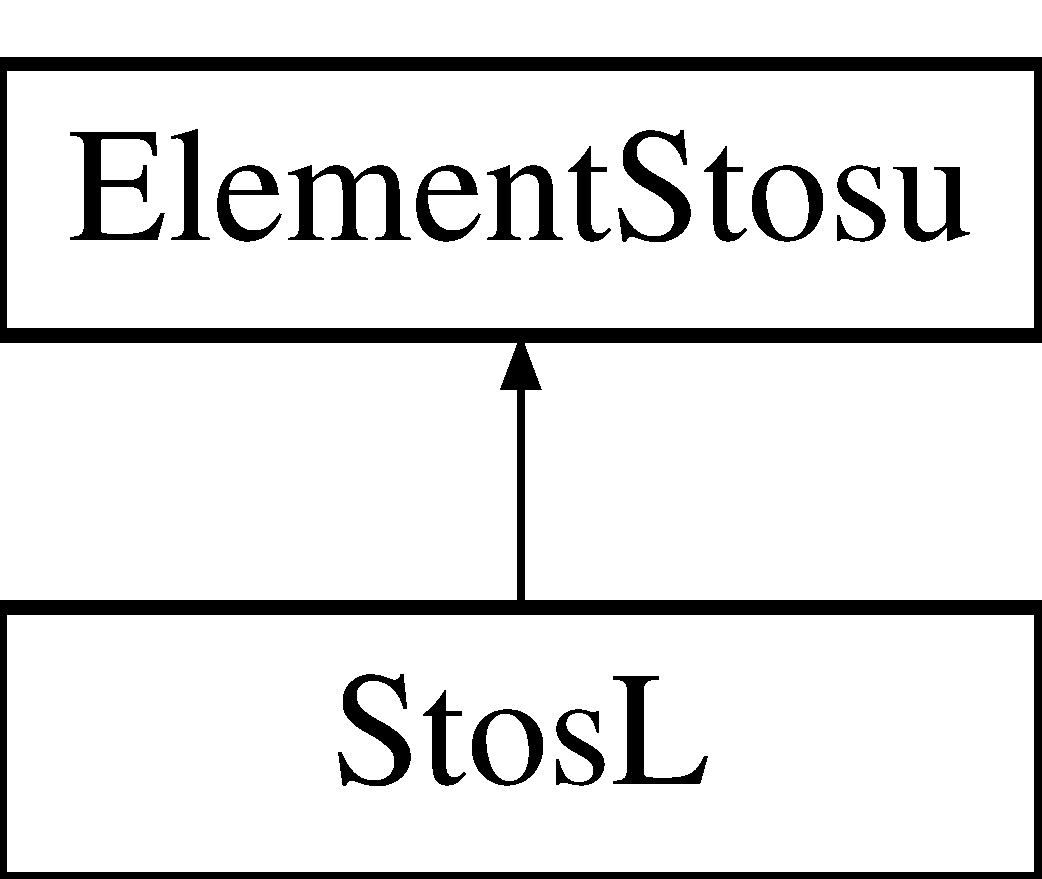
\includegraphics[height=2.000000cm]{class_stos_l}
\end{center}
\end{figure}
\subsection*{Metody publiczne}
\begin{DoxyCompactItemize}
\item 
void \hyperlink{class_stos_l_a429618cfa90a27679752faa885327218}{push} (int element)
\begin{DoxyCompactList}\small\item\em Funkcja dodajaca element do listy stosu. \end{DoxyCompactList}\item 
void \hyperlink{class_stos_l_aac10552d2133224615463be4a0e900c6}{pop} ()
\begin{DoxyCompactList}\small\item\em Funkcja usuwajaca ostatni element listy stosu. \end{DoxyCompactList}\item 
void \hyperlink{class_stos_l_a72dc2c599ac50911cd195d504ec397d6}{Wyswietl} ()
\begin{DoxyCompactList}\small\item\em Funkcja wyswietla cala liste stosu. \end{DoxyCompactList}\item 
\hyperlink{class_stos_l_adcf4ea69c11f7c501bbc85fa7cb1eabd}{Stos\-L} ()
\begin{DoxyCompactList}\small\item\em Konstrutktor klasy \hyperlink{class_stos_l}{Stos\-L}. \end{DoxyCompactList}\item 
int \hyperlink{class_stos_l_ad2bc9646e6994253c7804f83956fbc0f}{Top} ()
\begin{DoxyCompactList}\small\item\em Funkcja zwracajaca ostatni element stosu. \end{DoxyCompactList}\end{DoxyCompactItemize}
\subsection*{Atrybuty publiczne}
\begin{DoxyCompactItemize}
\item 
\hyperlink{class_element_stosu}{Element\-Stosu} $\ast$ \hyperlink{class_stos_l_a50de812f4b155571f88ea4ac6a0d5982}{pierwszy}
\begin{DoxyCompactList}\small\item\em Wskaznik na pierwszy element stosu. \end{DoxyCompactList}\end{DoxyCompactItemize}


\subsection{Opis szczegółowy}
Definicja klasy \hyperlink{class_stos_l}{Stos\-L} dziedziczaca klase \hyperlink{class_element_stosu}{Element\-Stosu}, majaca za zadanie dzialac na elementach stosu zaimplementowanego listowo. 

\subsection{Dokumentacja konstruktora i destruktora}
\hypertarget{class_stos_l_adcf4ea69c11f7c501bbc85fa7cb1eabd}{\index{Stos\-L@{Stos\-L}!Stos\-L@{Stos\-L}}
\index{Stos\-L@{Stos\-L}!StosL@{Stos\-L}}
\subsubsection[{Stos\-L}]{\setlength{\rightskip}{0pt plus 5cm}Stos\-L\-::\-Stos\-L (
\begin{DoxyParamCaption}
{}
\end{DoxyParamCaption}
)}}\label{class_stos_l_adcf4ea69c11f7c501bbc85fa7cb1eabd}


Konstrutktor klasy \hyperlink{class_stos_l}{Stos\-L}. 

Konstruktor ustawia wskaznik pierwszego elementu na zero (poniewaz na poczatku nie ma zadnych elementow). 

\subsection{Dokumentacja funkcji składowych}
\hypertarget{class_stos_l_aac10552d2133224615463be4a0e900c6}{\index{Stos\-L@{Stos\-L}!pop@{pop}}
\index{pop@{pop}!StosL@{Stos\-L}}
\subsubsection[{pop}]{\setlength{\rightskip}{0pt plus 5cm}void Stos\-L\-::pop (
\begin{DoxyParamCaption}
{}
\end{DoxyParamCaption}
)}}\label{class_stos_l_aac10552d2133224615463be4a0e900c6}


Funkcja usuwajaca ostatni element listy stosu. 

Parametry i najwazniejsza pola funkcji\-: -\/temp\-: wskaznik na obiekt \hyperlink{class_element_stosu}{Element\-Stosu}, ktory sluzy do znalezienia ostatniego elementu, ktory to bedzie usuniety (jego wartosc bedzie N\-U\-L\-L). \hypertarget{class_stos_l_a429618cfa90a27679752faa885327218}{\index{Stos\-L@{Stos\-L}!push@{push}}
\index{push@{push}!StosL@{Stos\-L}}
\subsubsection[{push}]{\setlength{\rightskip}{0pt plus 5cm}void Stos\-L\-::push (
\begin{DoxyParamCaption}
\item[{int}]{element}
\end{DoxyParamCaption}
)}}\label{class_stos_l_a429618cfa90a27679752faa885327218}


Funkcja dodajaca element do listy stosu. 

Parametry i najwazniejsza pola funkcji\-: -\/element\-: liczba typu int, ktora chcemy dodac do listy. -\/nowy\-: utworzony nowy obiekt \hyperlink{class_element_stosu}{Element\-Stosu}, ktory jest dodany na koniec listy stosu. -\/temp\-: utworzony przejsciowy wskaznik na obiekt \hyperlink{class_element_stosu}{Element\-Stosu} sluzacy do znalezienia ostatniego elementu i dodaniu na jego koniec wybranego.

Jesli jest pierwszym elementem listy, to staje sie poczatkiem listy. Jesli nie, po znalezieniu wskaznika na ostatni element, nowy element zastepuje ten ostatni. \hypertarget{class_stos_l_ad2bc9646e6994253c7804f83956fbc0f}{\index{Stos\-L@{Stos\-L}!Top@{Top}}
\index{Top@{Top}!StosL@{Stos\-L}}
\subsubsection[{Top}]{\setlength{\rightskip}{0pt plus 5cm}int Stos\-L\-::\-Top (
\begin{DoxyParamCaption}
{}
\end{DoxyParamCaption}
)}}\label{class_stos_l_ad2bc9646e6994253c7804f83956fbc0f}


Funkcja zwracajaca ostatni element stosu. 

\hypertarget{class_stos_l_a72dc2c599ac50911cd195d504ec397d6}{\index{Stos\-L@{Stos\-L}!Wyswietl@{Wyswietl}}
\index{Wyswietl@{Wyswietl}!StosL@{Stos\-L}}
\subsubsection[{Wyswietl}]{\setlength{\rightskip}{0pt plus 5cm}void Stos\-L\-::\-Wyswietl (
\begin{DoxyParamCaption}
{}
\end{DoxyParamCaption}
)}}\label{class_stos_l_a72dc2c599ac50911cd195d504ec397d6}


Funkcja wyswietla cala liste stosu. 



\subsection{Dokumentacja atrybutów składowych}
\hypertarget{class_stos_l_a50de812f4b155571f88ea4ac6a0d5982}{\index{Stos\-L@{Stos\-L}!pierwszy@{pierwszy}}
\index{pierwszy@{pierwszy}!StosL@{Stos\-L}}
\subsubsection[{pierwszy}]{\setlength{\rightskip}{0pt plus 5cm}{\bf Element\-Stosu}$\ast$ Stos\-L\-::pierwszy}}\label{class_stos_l_a50de812f4b155571f88ea4ac6a0d5982}


Wskaznik na pierwszy element stosu. 



Dokumentacja dla tej klasy została wygenerowana z plików\-:\begin{DoxyCompactItemize}
\item 
C\-:/\-Users/\-Witek/\-Documents/\-Visual Studio 2012/\-Projects/\-Project45\-P\-A\-M\-S\-Ilab5/\-Project45\-P\-A\-M\-S\-Ilab5/\hyperlink{_stos_l_8h}{Stos\-L.\-h}\item 
C\-:/\-Users/\-Witek/\-Documents/\-Visual Studio 2012/\-Projects/\-Project45\-P\-A\-M\-S\-Ilab5/\-Project45\-P\-A\-M\-S\-Ilab5/\hyperlink{_stos_l_8cpp}{Stos\-L.\-cpp}\end{DoxyCompactItemize}

\hypertarget{classtablica}{\section{Dokumentacja klasy tablica}
\label{classtablica}\index{tablica@{tablica}}
}


Deklaracja klasy tablica.  




{\ttfamily \#include $<$tablica.\-h$>$}

\subsection*{Metody publiczne}
\begin{DoxyCompactItemize}
\item 
int \hyperlink{classtablica_aa464212c27ab647f400f3d797dbc2a35}{Zwroc\-Ilosc\-Liczb} ()
\begin{DoxyCompactList}\small\item\em Funkcja zwracajaca ilosc liczb tablicy. \end{DoxyCompactList}\item 
void \hyperlink{classtablica_a5bcf67f378f0d78f29ec072d19f50e7c}{Pomnoz\-Liczby} (int liczba)
\begin{DoxyCompactList}\small\item\em Funkcja mnozaca liczby tablicy przez liczbe. \end{DoxyCompactList}\item 
void \hyperlink{classtablica_ad35970c518fe65267a08f80ac155b3b9}{Wyswietl\-Tablice} ()
\item 
\hyperlink{classtablica_a5453d2bbeeac4d81c1de4d3aedcb9855}{tablica} (char nazwa\mbox{[}$\,$\mbox{]})
\item 
\hyperlink{classtablica_abc5414ba4d6321ecf744e38a809d9c8f}{tablica} ()
\item 
void \hyperlink{classtablica_a066e82a4a56683dd01ad1b8de622ca84}{quicksort} (int p, int r)
\item 
void \hyperlink{classtablica_a12286c2881ab2db67e601b76c376f101}{sortuj\-\_\-babel} ()
\item 
void \hyperlink{classtablica_add56035c59826fba431fb0ea5252917d}{Zamien\-Elementy} (int i, int j)
\item 
void \hyperlink{classtablica_a6977d8d18f45c2939bbca7c4d3c54692}{Odwroc\-Kolejnosc} ()
\item 
void \hyperlink{classtablica_a68b5e30acd662df4f0eab6ffd4efc4b9}{Dodaj\-Element} (int element)
\item 
bool \hyperlink{classtablica_acc4a17a373df6ad19367830dd20d8db1}{operator==} (int tab\mbox{[}$\,$\mbox{]})
\item 
int $\ast$ \hyperlink{classtablica_acab922fa86307f71e4eb54d9ee51ec2f}{operator+} (\hyperlink{classtablica}{tablica} tab)
\item 
void \hyperlink{classtablica_af024511fa95d92e5fefd3d5fc075b6eb}{operator=} (\hyperlink{classtablica}{tablica} \&tabliczka)
\item 
void \hyperlink{classtablica_adfddb9569f480bd363e90660a72add95}{Wypelnij\-Stos\-Tablica} (\hyperlink{class_stos}{Stos} \&stosek)
\begin{DoxyCompactList}\small\item\em Funkcja, ktora po wczytaniu tablicy, kopiuje jej zawartosc do obiektu klasy \hyperlink{class_stos}{Stos}. \end{DoxyCompactList}\item 
void \hyperlink{classtablica_a888da3562ae1d3200c8ab446685f6c18}{Wypelnij\-Kolejke\-Tablica} (\hyperlink{class_kolejka}{Kolejka} \&kolejeczka)
\begin{DoxyCompactList}\small\item\em Funkcja, ktora po wczytaniu tablicy, kopiuje jej zawartosc do obiektu klasy \hyperlink{class_kolejka}{Kolejka}. \end{DoxyCompactList}\item 
void \hyperlink{classtablica_ae97c0bebf2629c77fa9c34a6aaf40d4f}{Wypelnij\-Stos\-L\-Tablica} (\hyperlink{class_stos_l}{Stos\-L} \&stosik\-L)
\begin{DoxyCompactList}\small\item\em Funkcja, ktora po wczytaniu tablicy, kopiuje jej zawartosc do obiektu klasy \hyperlink{class_stos_l}{Stos\-L}. \end{DoxyCompactList}\end{DoxyCompactItemize}
\subsection*{Atrybuty publiczne}
\begin{DoxyCompactItemize}
\item 
int $\ast$ \hyperlink{classtablica_ad6abcd9d60eef2315f0b92484058667b}{T\-A\-B\-L\-I\-C\-A}
\end{DoxyCompactItemize}


\subsection{Opis szczegółowy}
Deklaracja klasy tablica. 

Klasa tablica posiada pola oraz funkcje potrzebne do wykonywania dzialan na tablicach typu int. 

\subsection{Dokumentacja konstruktora i destruktora}
\hypertarget{classtablica_a5453d2bbeeac4d81c1de4d3aedcb9855}{\index{tablica@{tablica}!tablica@{tablica}}
\index{tablica@{tablica}!tablica@{tablica}}
\subsubsection[{tablica}]{\setlength{\rightskip}{0pt plus 5cm}tablica\-::tablica (
\begin{DoxyParamCaption}
\item[{char}]{nazwa\mbox{[}$\,$\mbox{]}}
\end{DoxyParamCaption}
)}}\label{classtablica_a5453d2bbeeac4d81c1de4d3aedcb9855}
Konstruktor klasy \hyperlink{class_operacja}{Operacja} tworzacy obiekt z tablica o okreslonej liczbie elementow.

Argumenty i najwazniejsze pola konstruktora\-:


\begin{DoxyItemize}
\item liczby -\/ ilosc liczb, ile zawierac bedzie glowna tablica po utworzeniu 
\end{DoxyItemize}\hypertarget{classtablica_abc5414ba4d6321ecf744e38a809d9c8f}{\index{tablica@{tablica}!tablica@{tablica}}
\index{tablica@{tablica}!tablica@{tablica}}
\subsubsection[{tablica}]{\setlength{\rightskip}{0pt plus 5cm}tablica\-::tablica (
\begin{DoxyParamCaption}
{}
\end{DoxyParamCaption}
)}}\label{classtablica_abc5414ba4d6321ecf744e38a809d9c8f}


\subsection{Dokumentacja funkcji składowych}
\hypertarget{classtablica_a68b5e30acd662df4f0eab6ffd4efc4b9}{\index{tablica@{tablica}!Dodaj\-Element@{Dodaj\-Element}}
\index{Dodaj\-Element@{Dodaj\-Element}!tablica@{tablica}}
\subsubsection[{Dodaj\-Element}]{\setlength{\rightskip}{0pt plus 5cm}void tablica\-::\-Dodaj\-Element (
\begin{DoxyParamCaption}
\item[{int}]{element}
\end{DoxyParamCaption}
)}}\label{classtablica_a68b5e30acd662df4f0eab6ffd4efc4b9}
Funkcja dodajaca wybrany element typu int do tablicy.

Argumenty i najwazniejsze pola funkcji\-:


\begin{DoxyItemize}
\item element -\/ wybrany element typu int, ktory chcemy dodac do tablicy
\item tabschow -\/ tablica, do ktorej zostanie zapisana nowa tablica z nowym elementem
\end{DoxyItemize}

\begin{DoxyReturn}{Zwraca}
Nowa tablica z dodanym elementem 
\end{DoxyReturn}
\hypertarget{classtablica_a6977d8d18f45c2939bbca7c4d3c54692}{\index{tablica@{tablica}!Odwroc\-Kolejnosc@{Odwroc\-Kolejnosc}}
\index{Odwroc\-Kolejnosc@{Odwroc\-Kolejnosc}!tablica@{tablica}}
\subsubsection[{Odwroc\-Kolejnosc}]{\setlength{\rightskip}{0pt plus 5cm}void tablica\-::\-Odwroc\-Kolejnosc (
\begin{DoxyParamCaption}
{}
\end{DoxyParamCaption}
)}}\label{classtablica_a6977d8d18f45c2939bbca7c4d3c54692}
Funkcja odwracajaca kolejnosc tablicy. \hypertarget{classtablica_acab922fa86307f71e4eb54d9ee51ec2f}{\index{tablica@{tablica}!operator+@{operator+}}
\index{operator+@{operator+}!tablica@{tablica}}
\subsubsection[{operator+}]{\setlength{\rightskip}{0pt plus 5cm}int $\ast$ tablica\-::operator+ (
\begin{DoxyParamCaption}
\item[{{\bf tablica}}]{tab}
\end{DoxyParamCaption}
)}}\label{classtablica_acab922fa86307f71e4eb54d9ee51ec2f}
Przeciazenie operatora dodawania (sklejania) dwoch tablic.

Argumenty i najwazniejsze pola funkcji\-:


\begin{DoxyItemize}
\item tab -\/ tablica, ktora bedzie dodana do glownej tablicy
\item tabschow -\/ tablica, do ktorej zostania zapisane dwie scalone tablice
\end{DoxyItemize}

\begin{DoxyReturn}{Zwraca}
Adres pierwszego elementu Nowej tablicy z dodana druga tablica 
\end{DoxyReturn}
\hypertarget{classtablica_af024511fa95d92e5fefd3d5fc075b6eb}{\index{tablica@{tablica}!operator=@{operator=}}
\index{operator=@{operator=}!tablica@{tablica}}
\subsubsection[{operator=}]{\setlength{\rightskip}{0pt plus 5cm}void tablica\-::operator= (
\begin{DoxyParamCaption}
\item[{{\bf tablica} \&}]{tabliczka}
\end{DoxyParamCaption}
)}}\label{classtablica_af024511fa95d92e5fefd3d5fc075b6eb}
Przeciazenie operatora przypisywania tablicy glownej innej tablicy.

\begin{DoxyVerb}            Przeciazenie to powoduje nadpisanie glownej tablicy wybrana tablica, zarazem zrownujac liczby elementow obu tablic.
\end{DoxyVerb}
 Argumenty i najwazniejsze pola funkcji\-:


\begin{DoxyItemize}
\item tab -\/ tablica, ktora nadpisze tablice glowna 
\end{DoxyItemize}\hypertarget{classtablica_acc4a17a373df6ad19367830dd20d8db1}{\index{tablica@{tablica}!operator==@{operator==}}
\index{operator==@{operator==}!tablica@{tablica}}
\subsubsection[{operator==}]{\setlength{\rightskip}{0pt plus 5cm}bool tablica\-::operator== (
\begin{DoxyParamCaption}
\item[{int}]{tab\mbox{[}$\,$\mbox{]}}
\end{DoxyParamCaption}
)}}\label{classtablica_acc4a17a373df6ad19367830dd20d8db1}
Przeciazenie operatora porownywania tablicy z tablic�.

Argumenty i najwazniejsze pola funkcji


\begin{DoxyItemize}
\item tab -\/ tablica wczytana jako pierwsza do porownania
\item prawda -\/ pole logiczne, przechowujace informacje o spelnionym warunku
\end{DoxyItemize}

\begin{DoxyReturn}{Zwraca}
prawda, jesli jest pelna zgodnosc; falsz, jesli wystapi blad w porownywaniu 
\end{DoxyReturn}
\hypertarget{classtablica_a5bcf67f378f0d78f29ec072d19f50e7c}{\index{tablica@{tablica}!Pomnoz\-Liczby@{Pomnoz\-Liczby}}
\index{Pomnoz\-Liczby@{Pomnoz\-Liczby}!tablica@{tablica}}
\subsubsection[{Pomnoz\-Liczby}]{\setlength{\rightskip}{0pt plus 5cm}void tablica\-::\-Pomnoz\-Liczby (
\begin{DoxyParamCaption}
\item[{int}]{liczba}
\end{DoxyParamCaption}
)}}\label{classtablica_a5bcf67f378f0d78f29ec072d19f50e7c}


Funkcja mnozaca liczby tablicy przez liczbe. 

Argumenty i najwazniejsze pola funkcji
\begin{DoxyItemize}
\item liczba -\/ liczba, przez ktora jest mnozony kazdy wyraz tablicy
\item tab\mbox{[}\mbox{]} -\/ tablica, na ktorej elementach bedzie wykonywane dzialanie
\item Ilosc -\/ ilosc danych wczytanych z pliku 
\end{DoxyItemize}\hypertarget{classtablica_a066e82a4a56683dd01ad1b8de622ca84}{\index{tablica@{tablica}!quicksort@{quicksort}}
\index{quicksort@{quicksort}!tablica@{tablica}}
\subsubsection[{quicksort}]{\setlength{\rightskip}{0pt plus 5cm}void tablica\-::quicksort (
\begin{DoxyParamCaption}
\item[{int}]{p, }
\item[{int}]{r}
\end{DoxyParamCaption}
)}}\label{classtablica_a066e82a4a56683dd01ad1b8de622ca84}
Funkcja wykonujaca algorytm quicksort. \hypertarget{classtablica_a12286c2881ab2db67e601b76c376f101}{\index{tablica@{tablica}!sortuj\-\_\-babel@{sortuj\-\_\-babel}}
\index{sortuj\-\_\-babel@{sortuj\-\_\-babel}!tablica@{tablica}}
\subsubsection[{sortuj\-\_\-babel}]{\setlength{\rightskip}{0pt plus 5cm}void tablica\-::sortuj\-\_\-babel (
\begin{DoxyParamCaption}
{}
\end{DoxyParamCaption}
)}}\label{classtablica_a12286c2881ab2db67e601b76c376f101}
Funkcja wykonujaca algorytm 'sortowania babelkowego'. \hypertarget{classtablica_a888da3562ae1d3200c8ab446685f6c18}{\index{tablica@{tablica}!Wypelnij\-Kolejke\-Tablica@{Wypelnij\-Kolejke\-Tablica}}
\index{Wypelnij\-Kolejke\-Tablica@{Wypelnij\-Kolejke\-Tablica}!tablica@{tablica}}
\subsubsection[{Wypelnij\-Kolejke\-Tablica}]{\setlength{\rightskip}{0pt plus 5cm}void tablica\-::\-Wypelnij\-Kolejke\-Tablica (
\begin{DoxyParamCaption}
\item[{{\bf Kolejka} \&}]{kolejeczka}
\end{DoxyParamCaption}
)}}\label{classtablica_a888da3562ae1d3200c8ab446685f6c18}


Funkcja, ktora po wczytaniu tablicy, kopiuje jej zawartosc do obiektu klasy \hyperlink{class_kolejka}{Kolejka}. 

\hypertarget{classtablica_ae97c0bebf2629c77fa9c34a6aaf40d4f}{\index{tablica@{tablica}!Wypelnij\-Stos\-L\-Tablica@{Wypelnij\-Stos\-L\-Tablica}}
\index{Wypelnij\-Stos\-L\-Tablica@{Wypelnij\-Stos\-L\-Tablica}!tablica@{tablica}}
\subsubsection[{Wypelnij\-Stos\-L\-Tablica}]{\setlength{\rightskip}{0pt plus 5cm}void tablica\-::\-Wypelnij\-Stos\-L\-Tablica (
\begin{DoxyParamCaption}
\item[{{\bf Stos\-L} \&}]{stosik\-L}
\end{DoxyParamCaption}
)}}\label{classtablica_ae97c0bebf2629c77fa9c34a6aaf40d4f}


Funkcja, ktora po wczytaniu tablicy, kopiuje jej zawartosc do obiektu klasy \hyperlink{class_stos_l}{Stos\-L}. 

\hypertarget{classtablica_adfddb9569f480bd363e90660a72add95}{\index{tablica@{tablica}!Wypelnij\-Stos\-Tablica@{Wypelnij\-Stos\-Tablica}}
\index{Wypelnij\-Stos\-Tablica@{Wypelnij\-Stos\-Tablica}!tablica@{tablica}}
\subsubsection[{Wypelnij\-Stos\-Tablica}]{\setlength{\rightskip}{0pt plus 5cm}void tablica\-::\-Wypelnij\-Stos\-Tablica (
\begin{DoxyParamCaption}
\item[{{\bf Stos} \&}]{stosek}
\end{DoxyParamCaption}
)}}\label{classtablica_adfddb9569f480bd363e90660a72add95}


Funkcja, ktora po wczytaniu tablicy, kopiuje jej zawartosc do obiektu klasy \hyperlink{class_stos}{Stos}. 

\hypertarget{classtablica_ad35970c518fe65267a08f80ac155b3b9}{\index{tablica@{tablica}!Wyswietl\-Tablice@{Wyswietl\-Tablice}}
\index{Wyswietl\-Tablice@{Wyswietl\-Tablice}!tablica@{tablica}}
\subsubsection[{Wyswietl\-Tablice}]{\setlength{\rightskip}{0pt plus 5cm}void tablica\-::\-Wyswietl\-Tablice (
\begin{DoxyParamCaption}
{}
\end{DoxyParamCaption}
)}}\label{classtablica_ad35970c518fe65267a08f80ac155b3b9}
Funkcja wyswietlajaca wyrazy tablicy klasy \hyperlink{class_operacja}{Operacja}.

Funkcja wyswietla wszystkie elementy tablicy glownej w zaleznosci od przechowywanej w polu Ilosc\-Liczb informacji o liczbie jej elementow. \hypertarget{classtablica_add56035c59826fba431fb0ea5252917d}{\index{tablica@{tablica}!Zamien\-Elementy@{Zamien\-Elementy}}
\index{Zamien\-Elementy@{Zamien\-Elementy}!tablica@{tablica}}
\subsubsection[{Zamien\-Elementy}]{\setlength{\rightskip}{0pt plus 5cm}void tablica\-::\-Zamien\-Elementy (
\begin{DoxyParamCaption}
\item[{int}]{i, }
\item[{int}]{j}
\end{DoxyParamCaption}
)}}\label{classtablica_add56035c59826fba431fb0ea5252917d}
Funkcja zamieniajaca miejscami wybrane elementy tablicy.

Argumenty i najwazniejsze pola funkcji\-:


\begin{DoxyItemize}
\item i -\/ wybrany element pierwszej tablicy
\item j -\/ wybrany element drugiej tablicy 
\end{DoxyItemize}\hypertarget{classtablica_aa464212c27ab647f400f3d797dbc2a35}{\index{tablica@{tablica}!Zwroc\-Ilosc\-Liczb@{Zwroc\-Ilosc\-Liczb}}
\index{Zwroc\-Ilosc\-Liczb@{Zwroc\-Ilosc\-Liczb}!tablica@{tablica}}
\subsubsection[{Zwroc\-Ilosc\-Liczb}]{\setlength{\rightskip}{0pt plus 5cm}int tablica\-::\-Zwroc\-Ilosc\-Liczb (
\begin{DoxyParamCaption}
{}
\end{DoxyParamCaption}
)}}\label{classtablica_aa464212c27ab647f400f3d797dbc2a35}


Funkcja zwracajaca ilosc liczb tablicy. 



\subsection{Dokumentacja atrybutów składowych}
\hypertarget{classtablica_ad6abcd9d60eef2315f0b92484058667b}{\index{tablica@{tablica}!T\-A\-B\-L\-I\-C\-A@{T\-A\-B\-L\-I\-C\-A}}
\index{T\-A\-B\-L\-I\-C\-A@{T\-A\-B\-L\-I\-C\-A}!tablica@{tablica}}
\subsubsection[{T\-A\-B\-L\-I\-C\-A}]{\setlength{\rightskip}{0pt plus 5cm}int$\ast$ tablica\-::\-T\-A\-B\-L\-I\-C\-A}}\label{classtablica_ad6abcd9d60eef2315f0b92484058667b}
Pole przechowujace glowna tablice klasy \hyperlink{class_operacja}{Operacja}. 

Dokumentacja dla tej klasy została wygenerowana z plików\-:\begin{DoxyCompactItemize}
\item 
C\-:/\-Users/\-Witek/\-Documents/\-Visual Studio 2012/\-Projects/\-Project44\-P\-A\-M\-S\-Ilab3/\-Project44\-P\-A\-M\-S\-Ilab3/\hyperlink{tablica_8h}{tablica.\-h}\item 
C\-:/\-Users/\-Witek/\-Documents/\-Visual Studio 2012/\-Projects/\-Project44\-P\-A\-M\-S\-Ilab3/\-Project44\-P\-A\-M\-S\-Ilab3/\hyperlink{tablica_8cpp}{tablica.\-cpp}\end{DoxyCompactItemize}

\chapter{Dokumentacja plików}
\hypertarget{_kolejka_8cpp}{\section{Dokumentacja pliku C\-:/\-Users/\-Witek/\-Documents/\-Visual Studio 2012/\-Projects/\-Project45\-P\-A\-M\-S\-Ilab4/\-Project44\-P\-A\-M\-S\-Ilab4/\-Kolejka.cpp}
\label{_kolejka_8cpp}\index{C\-:/\-Users/\-Witek/\-Documents/\-Visual Studio 2012/\-Projects/\-Project45\-P\-A\-M\-S\-Ilab4/\-Project44\-P\-A\-M\-S\-Ilab4/\-Kolejka.\-cpp@{C\-:/\-Users/\-Witek/\-Documents/\-Visual Studio 2012/\-Projects/\-Project45\-P\-A\-M\-S\-Ilab4/\-Project44\-P\-A\-M\-S\-Ilab4/\-Kolejka.\-cpp}}
}
{\ttfamily \#include $<$iostream$>$}\\*
{\ttfamily \#include \char`\"{}Kolejka.\-h\char`\"{}}\\*

\hypertarget{_kolejka_8h}{\section{Dokumentacja pliku C\-:/\-Users/\-Witek/\-Documents/\-Visual Studio 2012/\-Projects/\-Project45\-P\-A\-M\-S\-Ilab4/\-Project44\-P\-A\-M\-S\-Ilab4/\-Kolejka.h}
\label{_kolejka_8h}\index{C\-:/\-Users/\-Witek/\-Documents/\-Visual Studio 2012/\-Projects/\-Project45\-P\-A\-M\-S\-Ilab4/\-Project44\-P\-A\-M\-S\-Ilab4/\-Kolejka.\-h@{C\-:/\-Users/\-Witek/\-Documents/\-Visual Studio 2012/\-Projects/\-Project45\-P\-A\-M\-S\-Ilab4/\-Project44\-P\-A\-M\-S\-Ilab4/\-Kolejka.\-h}}
}
{\ttfamily \#include $<$iostream$>$}\\*
\subsection*{Komponenty}
\begin{DoxyCompactItemize}
\item 
class \hyperlink{class_kolejka}{Kolejka}
\begin{DoxyCompactList}\small\item\em Definicja klasy \hyperlink{class_kolejka}{Kolejka}. \end{DoxyCompactList}\end{DoxyCompactItemize}

\hypertarget{main_8cpp}{\section{Dokumentacja pliku C\-:/\-Users/\-Witek/\-Documents/\-Visual Studio 2012/\-Projects/\-Project48\-P\-A\-M\-S\-Ilab8/\-Project48\-P\-A\-M\-S\-Ilab8/main.cpp}
\label{main_8cpp}\index{C\-:/\-Users/\-Witek/\-Documents/\-Visual Studio 2012/\-Projects/\-Project48\-P\-A\-M\-S\-Ilab8/\-Project48\-P\-A\-M\-S\-Ilab8/main.\-cpp@{C\-:/\-Users/\-Witek/\-Documents/\-Visual Studio 2012/\-Projects/\-Project48\-P\-A\-M\-S\-Ilab8/\-Project48\-P\-A\-M\-S\-Ilab8/main.\-cpp}}
}
{\ttfamily \#include \char`\"{}operacja.\-h\char`\"{}}\\*
\subsection*{Funkcje}
\begin{DoxyCompactItemize}
\item 
int \hyperlink{main_8cpp_ae66f6b31b5ad750f1fe042a706a4e3d4}{main} ()
\begin{DoxyCompactList}\small\item\em Funkcja main wykonujaca wyszukiwanie sciezek w grafie i liczaca czasy. \end{DoxyCompactList}\end{DoxyCompactItemize}


\subsection{Dokumentacja funkcji}
\hypertarget{main_8cpp_ae66f6b31b5ad750f1fe042a706a4e3d4}{\index{main.\-cpp@{main.\-cpp}!main@{main}}
\index{main@{main}!main.cpp@{main.\-cpp}}
\subsubsection[{main}]{\setlength{\rightskip}{0pt plus 5cm}int main (
\begin{DoxyParamCaption}
{}
\end{DoxyParamCaption}
)}}\label{main_8cpp_ae66f6b31b5ad750f1fe042a706a4e3d4}


Funkcja main wykonujaca wyszukiwanie sciezek w grafie i liczaca czasy. 

W funkcji main wykonywane sa nastepujace operacje\-:


\begin{DoxyItemize}
\item Tworzony jest obiekt klasy \hyperlink{class_operacja}{Operacja}
\item Uruchamiany jest interfejs i mozliwe jest wybranie algorytmu przeszukiwania grafu, ktory chcemy obserwowac. 
\end{DoxyItemize}
\hypertarget{operacja_8cpp}{\section{Dokumentacja pliku C\-:/\-Users/\-Witek/\-Documents/\-Visual Studio 2012/\-Projects/\-Project48\-P\-A\-M\-S\-Ilab8/\-Project48\-P\-A\-M\-S\-Ilab8/operacja.cpp}
\label{operacja_8cpp}\index{C\-:/\-Users/\-Witek/\-Documents/\-Visual Studio 2012/\-Projects/\-Project48\-P\-A\-M\-S\-Ilab8/\-Project48\-P\-A\-M\-S\-Ilab8/operacja.\-cpp@{C\-:/\-Users/\-Witek/\-Documents/\-Visual Studio 2012/\-Projects/\-Project48\-P\-A\-M\-S\-Ilab8/\-Project48\-P\-A\-M\-S\-Ilab8/operacja.\-cpp}}
}
{\ttfamily \#include \char`\"{}operacja.\-h\char`\"{}}\\*
{\ttfamily \#include $<$string$>$}\\*

\hypertarget{operacja_8h}{\section{Dokumentacja pliku C\-:/\-Users/\-Witek/\-Documents/\-Visual Studio 2012/\-Projects/\-Project43\-P\-A\-M\-S\-Ilab2/\-Project43\-P\-A\-M\-S\-Ilab2/operacja.h}
\label{operacja_8h}\index{C\-:/\-Users/\-Witek/\-Documents/\-Visual Studio 2012/\-Projects/\-Project43\-P\-A\-M\-S\-Ilab2/\-Project43\-P\-A\-M\-S\-Ilab2/operacja.\-h@{C\-:/\-Users/\-Witek/\-Documents/\-Visual Studio 2012/\-Projects/\-Project43\-P\-A\-M\-S\-Ilab2/\-Project43\-P\-A\-M\-S\-Ilab2/operacja.\-h}}
}
{\ttfamily \#include $<$iostream$>$}\\*
{\ttfamily \#include $<$fstream$>$}\\*
{\ttfamily \#include $<$ctime$>$}\\*
\subsection*{Komponenty}
\begin{DoxyCompactItemize}
\item 
class \hyperlink{class_operacja}{Operacja}
\begin{DoxyCompactList}\small\item\em Deklaracja klasy \hyperlink{class_operacja}{Operacja}. \end{DoxyCompactList}\end{DoxyCompactItemize}
\subsection*{Funkcje}
\begin{DoxyCompactItemize}
\item 
void \hyperlink{operacja_8h_a4f45ead62a93f12bf227fae7303fb5d4}{Wyswietl\-Tablice} (int tab\mbox{[}$\,$\mbox{]}, int Ilosc)
\end{DoxyCompactItemize}


\subsection{Dokumentacja funkcji}
\hypertarget{operacja_8h_a4f45ead62a93f12bf227fae7303fb5d4}{\index{operacja.\-h@{operacja.\-h}!Wyswietl\-Tablice@{Wyswietl\-Tablice}}
\index{Wyswietl\-Tablice@{Wyswietl\-Tablice}!operacja.h@{operacja.\-h}}
\subsubsection[{Wyswietl\-Tablice}]{\setlength{\rightskip}{0pt plus 5cm}void Wyswietl\-Tablice (
\begin{DoxyParamCaption}
\item[{int}]{tab\mbox{[}$\,$\mbox{]}, }
\item[{int}]{Ilosc}
\end{DoxyParamCaption}
)}}\label{operacja_8h_a4f45ead62a93f12bf227fae7303fb5d4}
Funkcja pomocnicza wyswietlajaca wyrazy dowolnej tablicy w zaleznosci od ilosci jej elementow.

Funkcja wyswietlajaca nie tylko tablice z klasy \hyperlink{class_operacja}{Operacja}, lecz kazda inna o zadanej ilosci elementow Argumenty i najwazniejsze pola funkcji


\begin{DoxyItemize}
\item tab\mbox{[}\mbox{]} -\/ tablica, ktora jest wyswietlana
\item Ilosc -\/ ilosc danych do wyswietlenia 
\end{DoxyItemize}
\hypertarget{_stos_8cpp}{\section{Dokumentacja pliku C\-:/\-Users/\-Witek/\-Documents/\-Visual Studio 2012/\-Projects/\-Project45\-P\-A\-M\-S\-Ilab4/\-Project44\-P\-A\-M\-S\-Ilab4/\-Stos.cpp}
\label{_stos_8cpp}\index{C\-:/\-Users/\-Witek/\-Documents/\-Visual Studio 2012/\-Projects/\-Project45\-P\-A\-M\-S\-Ilab4/\-Project44\-P\-A\-M\-S\-Ilab4/\-Stos.\-cpp@{C\-:/\-Users/\-Witek/\-Documents/\-Visual Studio 2012/\-Projects/\-Project45\-P\-A\-M\-S\-Ilab4/\-Project44\-P\-A\-M\-S\-Ilab4/\-Stos.\-cpp}}
}
{\ttfamily \#include $<$iostream$>$}\\*
{\ttfamily \#include $<$fstream$>$}\\*
{\ttfamily \#include \char`\"{}Stos.\-h\char`\"{}}\\*

\hypertarget{_stos_8h}{\section{Dokumentacja pliku C\-:/\-Users/\-Witek/\-Documents/\-Visual Studio 2012/\-Projects/\-Project44\-P\-A\-M\-S\-Ilab3/\-Project44\-P\-A\-M\-S\-Ilab3/\-Stos.h}
\label{_stos_8h}\index{C\-:/\-Users/\-Witek/\-Documents/\-Visual Studio 2012/\-Projects/\-Project44\-P\-A\-M\-S\-Ilab3/\-Project44\-P\-A\-M\-S\-Ilab3/\-Stos.\-h@{C\-:/\-Users/\-Witek/\-Documents/\-Visual Studio 2012/\-Projects/\-Project44\-P\-A\-M\-S\-Ilab3/\-Project44\-P\-A\-M\-S\-Ilab3/\-Stos.\-h}}
}
{\ttfamily \#include $<$iostream$>$}\\*
{\ttfamily \#include $<$stack$>$}\\*
\subsection*{Komponenty}
\begin{DoxyCompactItemize}
\item 
class \hyperlink{class_stos}{Stos}
\begin{DoxyCompactList}\small\item\em Definicja klasy \hyperlink{class_stos}{Stos} implementowanej tablicowo. \end{DoxyCompactList}\end{DoxyCompactItemize}

\hypertarget{_stos_l_8cpp}{\section{Dokumentacja pliku C\-:/\-Users/\-Witek/\-Documents/\-Visual Studio 2012/\-Projects/\-Project45\-P\-A\-M\-S\-Ilab4/\-Project44\-P\-A\-M\-S\-Ilab4/\-Stos\-L.cpp}
\label{_stos_l_8cpp}\index{C\-:/\-Users/\-Witek/\-Documents/\-Visual Studio 2012/\-Projects/\-Project45\-P\-A\-M\-S\-Ilab4/\-Project44\-P\-A\-M\-S\-Ilab4/\-Stos\-L.\-cpp@{C\-:/\-Users/\-Witek/\-Documents/\-Visual Studio 2012/\-Projects/\-Project45\-P\-A\-M\-S\-Ilab4/\-Project44\-P\-A\-M\-S\-Ilab4/\-Stos\-L.\-cpp}}
}
{\ttfamily \#include $<$iostream$>$}\\*
{\ttfamily \#include \char`\"{}Stos\-L.\-h\char`\"{}}\\*

\hypertarget{_stos_l_8h}{\section{Dokumentacja pliku C\-:/\-Users/\-Witek/\-Documents/\-Visual Studio 2012/\-Projects/\-Project45\-P\-A\-M\-S\-Ilab5/\-Project45\-P\-A\-M\-S\-Ilab5/\-Stos\-L.h}
\label{_stos_l_8h}\index{C\-:/\-Users/\-Witek/\-Documents/\-Visual Studio 2012/\-Projects/\-Project45\-P\-A\-M\-S\-Ilab5/\-Project45\-P\-A\-M\-S\-Ilab5/\-Stos\-L.\-h@{C\-:/\-Users/\-Witek/\-Documents/\-Visual Studio 2012/\-Projects/\-Project45\-P\-A\-M\-S\-Ilab5/\-Project45\-P\-A\-M\-S\-Ilab5/\-Stos\-L.\-h}}
}
{\ttfamily \#include $<$iostream$>$}\\*
\subsection*{Komponenty}
\begin{DoxyCompactItemize}
\item 
class \hyperlink{class_element_stosu}{Element\-Stosu}
\begin{DoxyCompactList}\small\item\em Definicja klasy \hyperlink{class_element_stosu}{Element\-Stosu} , opisujacej jeden z listowej implementacji klasy \hyperlink{class_stos_l}{Stos\-L}. \end{DoxyCompactList}\item 
class \hyperlink{class_stos_l}{Stos\-L}
\begin{DoxyCompactList}\small\item\em Definicja klasy \hyperlink{class_stos_l}{Stos\-L} dziedziczaca klase \hyperlink{class_element_stosu}{Element\-Stosu}, majaca za zadanie dzialac na elementach stosu zaimplementowanego listowo. \end{DoxyCompactList}\end{DoxyCompactItemize}

\hypertarget{tablica_8cpp}{\section{Dokumentacja pliku C\-:/\-Users/\-Witek/\-Documents/\-Visual Studio 2012/\-Projects/\-Project45\-P\-A\-M\-S\-Ilab5/\-Project45\-P\-A\-M\-S\-Ilab5/tablica.cpp}
\label{tablica_8cpp}\index{C\-:/\-Users/\-Witek/\-Documents/\-Visual Studio 2012/\-Projects/\-Project45\-P\-A\-M\-S\-Ilab5/\-Project45\-P\-A\-M\-S\-Ilab5/tablica.\-cpp@{C\-:/\-Users/\-Witek/\-Documents/\-Visual Studio 2012/\-Projects/\-Project45\-P\-A\-M\-S\-Ilab5/\-Project45\-P\-A\-M\-S\-Ilab5/tablica.\-cpp}}
}
{\ttfamily \#include \char`\"{}tablica.\-h\char`\"{}}\\*
{\ttfamily \#include $<$iostream$>$}\\*
{\ttfamily \#include $<$fstream$>$}\\*
{\ttfamily \#include $<$ctime$>$}\\*
\subsection*{Funkcje}
\begin{DoxyCompactItemize}
\item 
void \hyperlink{tablica_8cpp_a4f45ead62a93f12bf227fae7303fb5d4}{Wyswietl\-Tablice} (int tab\mbox{[}$\,$\mbox{]}, int Ilosc)
\end{DoxyCompactItemize}


\subsection{Dokumentacja funkcji}
\hypertarget{tablica_8cpp_a4f45ead62a93f12bf227fae7303fb5d4}{\index{tablica.\-cpp@{tablica.\-cpp}!Wyswietl\-Tablice@{Wyswietl\-Tablice}}
\index{Wyswietl\-Tablice@{Wyswietl\-Tablice}!tablica.cpp@{tablica.\-cpp}}
\subsubsection[{Wyswietl\-Tablice}]{\setlength{\rightskip}{0pt plus 5cm}void Wyswietl\-Tablice (
\begin{DoxyParamCaption}
\item[{int}]{tab\mbox{[}$\,$\mbox{]}, }
\item[{int}]{Ilosc}
\end{DoxyParamCaption}
)}}\label{tablica_8cpp_a4f45ead62a93f12bf227fae7303fb5d4}
Funkcja wyswietlajaca nie tylko tablice z klasy \hyperlink{class_operacja}{Operacja}, lecz kazda inna o zadanej ilosci elementow Argumenty i najwazniejsze pola funkcji


\begin{DoxyItemize}
\item tab\mbox{[}\mbox{]} -\/ tablica, ktora jest wyswietlana
\item Ilosc -\/ ilosc danych do wyswietlenia 
\end{DoxyItemize}
\hypertarget{tablica_8h}{\section{Dokumentacja pliku C\-:/\-Users/\-Witek/\-Documents/\-Visual Studio 2012/\-Projects/\-Project45\-P\-A\-M\-S\-Ilab5/\-Project45\-P\-A\-M\-S\-Ilab5/tablica.h}
\label{tablica_8h}\index{C\-:/\-Users/\-Witek/\-Documents/\-Visual Studio 2012/\-Projects/\-Project45\-P\-A\-M\-S\-Ilab5/\-Project45\-P\-A\-M\-S\-Ilab5/tablica.\-h@{C\-:/\-Users/\-Witek/\-Documents/\-Visual Studio 2012/\-Projects/\-Project45\-P\-A\-M\-S\-Ilab5/\-Project45\-P\-A\-M\-S\-Ilab5/tablica.\-h}}
}
{\ttfamily \#include $<$iostream$>$}\\*
{\ttfamily \#include \char`\"{}Stos.\-h\char`\"{}}\\*
{\ttfamily \#include \char`\"{}Kolejka.\-h\char`\"{}}\\*
{\ttfamily \#include \char`\"{}Stos\-L.\-h\char`\"{}}\\*
\subsection*{Komponenty}
\begin{DoxyCompactItemize}
\item 
class \hyperlink{classtablica}{tablica}
\begin{DoxyCompactList}\small\item\em Deklaracja klasy tablica. \end{DoxyCompactList}\end{DoxyCompactItemize}
\subsection*{Funkcje}
\begin{DoxyCompactItemize}
\item 
void \hyperlink{tablica_8h_a4f45ead62a93f12bf227fae7303fb5d4}{Wyswietl\-Tablice} (int tab\mbox{[}$\,$\mbox{]}, int Ilosc)
\end{DoxyCompactItemize}


\subsection{Dokumentacja funkcji}
\hypertarget{tablica_8h_a4f45ead62a93f12bf227fae7303fb5d4}{\index{tablica.\-h@{tablica.\-h}!Wyswietl\-Tablice@{Wyswietl\-Tablice}}
\index{Wyswietl\-Tablice@{Wyswietl\-Tablice}!tablica.h@{tablica.\-h}}
\subsubsection[{Wyswietl\-Tablice}]{\setlength{\rightskip}{0pt plus 5cm}void Wyswietl\-Tablice (
\begin{DoxyParamCaption}
\item[{int}]{tab\mbox{[}$\,$\mbox{]}, }
\item[{int}]{Ilosc}
\end{DoxyParamCaption}
)}}\label{tablica_8h_a4f45ead62a93f12bf227fae7303fb5d4}
Funkcja pomocnicza wyswietlajaca wyrazy dowolnej tablicy w zaleznosci od ilosci jej elementow.

Funkcja wyswietlajaca nie tylko tablice z klasy \hyperlink{class_operacja}{Operacja}, lecz kazda inna o zadanej ilosci elementow Argumenty i najwazniejsze pola funkcji


\begin{DoxyItemize}
\item tab\mbox{[}\mbox{]} -\/ tablica, ktora jest wyswietlana
\item Ilosc -\/ ilosc danych do wyswietlenia 
\end{DoxyItemize}
\printindex
\end{document}
